\begin{exercises} 

\item \label{Ez:9.8.1}    Consider the moving particle whose position at time $t$ in seconds is given by the vector-valued function $\vr$ defined by $\vr(t) = 5t \vi + 4\sin(3t) \vj + 4\cos(3t) \vk$.  Use this function to answer each of the following questions. 
				
    \ba
   	\item Find the unit tangent vector, $\vT(t)$, to the spacecurve traced by $\vr(t)$ at time $t$.  Write one sentence that explains what $\vT(t)$ tells us about the particle's motion.
     	\item Determine the speed of the particle moving along the spacecurve with the given parameterization.
	\item Find the exact distance traveled by the particle on the time interval $[0,\pi/3]$.
	\item Find the average velocity of the particle on the time interval $[0, \pi/3]$.
	\item Determine the parameterization of the given curve with respect to arc length.
    \ea


\begin{exerciseSolution}
 \ba
   	\item The unit tangent vector $\vT(t)$ is found as 
\[\vT(t) = \frac{\vr'(t)}{|\vr'(t)|} = \frac{1}{\sqrt{13}}(5 \vi + 12\cos(3t) \vj - 12\sin(3t) \vk).\]
The unit tangent vector $\vT(t)$ tells us the direction of motion of the particle at time $t$. 
    \item The speed of the particle is the magnitude of the velocity vector, so the speed of the particle at time $t$ is 
    \[|\vr'(t)| = 13.\]
So the particle is moving at a constant speed. 
	\item The distance traveled by the particle on a time interval $[a,b]$ is the length of the arc on $[a,b]$. In this case, the exact distance traveled by the particle on the time interval $[0,\pi/3]$ is
	\[\int_0^{\pi/3} |\vr'(t)| \, dt = \int_0^{\pi/3} 13 \, dt = \frac{13 \pi}{3}.\]
	\item The average velocity of the particle on the time interval $[0, \pi/3]$ is
	\[\frac{1}{\pi/3} (\vr(\pi/3) - \vr(0)) = \frac{3}{\pi} \left\langle \frac{5 \pi}{3}, 0, -8 \right\rangle.\] 
	\item The arclength from $0$ to $t$ is 
\[s = L(t) = \int_0^t |\vr'(w)| \, dw = 13 t,\]
so $t = L^{-1}(s) = \frac{1}{13}s$. Therefore, a parameterization of the curve with respect to arc length is
\[\vr(s) = \vr\left(\frac{1}{13}s\right) =  \frac{5}{13}s \vi + 4\sin\left(\frac{3}{13}s\right) \vj + 4\cos\left(\frac{3}{13}s\right) \vk.\]
    \ea
\end{exerciseSolution}


\item \label{Ez:9.8.2} Let $y = f(x)$ define a curve in the plane. We can consider this curve as a curve in three-space with $z$-coordinate 0. 
	\ba
	\item Find a parameterization of the form $\vr(t) = \langle x(t), y(t), z(t) \rangle$ of the curve $y=f(x)$ in three-space. 
	\item Use the formula 
\[\kappa = \frac{\lvert \vr'(t) \times \vr''(t) \rvert}{\lvert \vr'(t) \rvert^3}\]
to show that 
\[\kappa = \frac{\lvert f''(x) \rvert}{\left[1+(f'(x))^2\right]^{3/2}}.\]
	\ea

\begin{exerciseSolution}
    \ba
	    \item If we let $x(t) = t$, then $y(t) = f(t)$ and $z(t)=0$. So a parameterization of the curve defined by $y=f(x)$ is 
\[\vr(t) = \langle t, f(t), 0 \rangle.\]
	    \item Since 
	    \[\vr'(t) = \vi + f'(t) \vj \text{ and } \vr''(t) = f''(t) \vj,\]
	    we have 
	    \[\vr'(t) \times \vr''(t) = f''(t) \vk.\]
	    So 
\begin{align*}
\kappa &= \frac{\lvert \vr'(t) \times \vr''(t) \rvert}{\lvert \vr'(t) \rvert^3} \\
	&= \frac{\lvert f''(t) \rvert}{\sqrt{1+(f'(t))^2}^3} \\
	&= \frac{\lvert f''(t) \rvert}{\left[1+(f'(t))^2\right]^{3/2}}.
\end{align*}
    \ea
\end{exerciseSolution}	

	
\item \label{Ez:9.8.3}    Consider the single variable function $y = 4x^2 - x^3.$ 
    \ba
	    \item Find a parameterization of the form $\vr(t) = \langle x(t), y(t) \rangle$ that traces the curve $y = 4x^2 - x^3$ on the interval from $x =  -3$ to $x = 3$.
	    \item Write a definite integral which, if evaluated, gives the exact length of the given curve from $x =  -3$ to $x = 3$.  Why is the integral difficult to evaluate exactly?
	    \item Determine the curvature, $\kappa(t)$, of the parameterized curve. (Exercise \ref{Ez:9.8.2} might be useful here.)
	    \item Use appropriate technology to approximate the absolute maximum and minimum of $\kappa(t)$ on the parameter interval for your parameterization.  Compare your results with the graph of $y = 4x^2 - x^3$.  How do the absolute maximum and absolute minimum of $\kappa(t)$ align with the original curve?
    \ea


\begin{exerciseSolution}
    \ba
	    \item If we let $x(t) = t$, then $y(t) = 4t^2-t^3$. So a parameterization of the curve on the interval from $x =  -3$ to $x = 3$ is
\[\vr(t) = \langle t, 4t^2-t^3 \rangle\]
for $t$ in $[-3,3]$. 
	    \item The length of the curve for $x =  -3$ to $x = 3$ is given by the integral
\[\int_{-3}^{3} |\vr'(t)| \, dt = \int_{-3}^3 \sqrt{1+(8t-3t^2)^2} \, dt.\]
The sum under the root makes this integral difficult to evaluate exactly.
	    \item The curvature $\kappa(t)$ can be calculated using the formula from Exercise \ref{Ez:9.8.2}. Since $f'(x) = 8x - 3x^2$ and $f''(x) = 8-6x$, we have 
\[\kappa(t) = \frac{ \lvert 8-6t \rvert }{ \left[1+(8t-3t^2)^2\right]^{3/2} }.\]
	    \item A plot of $\kappa(t)$ on the interval $[-3,3]$ shows relative maxima near 0 and 2.8. A computer algebra system shows that $\frac{ 8-6t  }{ \left[1+(8t-3t^2)^2\right]^{3/2} }$ has critical numbers at approximately $-0.003881710157$ and $2.670548377$. Now 
\[\kappa(-0.003881710157) \approx  8.011664828 \text{ and } \kappa(2.670548377) \approx 8.011664851,\]
so the maximum value of $\kappa$ on $[-3,3]$ is approximately 8.011664851. The minimum value of $\kappa$ must occur at an endpoint. Since 
\[\kappa(-3) \approx 0.0001958900647 \text{ and } \kappa(3) \approx 0.3162277660,\]
the minimum value of $\kappa$ on $[-3,3]$ is approximately 0.0001958900647. The graph of $y=4x^2-x^3$ is close to linear at $x=-3$, which accounts for the low value of $\kappa$ there. The largest curvature in the graph is  just after the critical point at $x = \frac{8}{3} \approx 2.666$.  
    \ea
\end{exerciseSolution}


\item \label{Ez:9.8.4}    Consider the standard helix parameterized by $\vr(t) = \cos(t) \vi + \sin(t) \vj + t \vk$.
    \ba
	    \item Recall that the unit tangent vector, $\vT(t)$, is the vector tangent to the curve at time $t$ that points in the direction of motion and has length 1.  Find $\vT(t)$.
	    \item Explain why the fact that $| \vT(t) | = 1$ implies that $\vT$ and $\vT'$ are orthogonal vectors for every value of $t$.  (Hint:  note that $\vT \cdot \vT = |\vT|^2 = 1,$ and compute $\frac{d}{dt}[\vT \cdot \vT]$.)
	    \item For the given function $\vr(t)$ with unit tangent vector $\vT(t)$ (from (a)), determine $\vN(t) = \frac{1}{|\vT'(t)|} \vT'(t)$.
	    \item What geometric properties does $\vN(t)$ have?  That is, how long is this vector, and how is it situated in comparison to $\vT(t)$?
	    \item Let $\vB(t) = \vT(t) \times \vN(t)$, and compute $\vB(t)$ in terms of your results in (a) and (c).
	    \item What geometric properties does $\vB(t)$ have?  That is, how long is this vector, and how is it situated in comparison to $\vT(t)$ and $\vN(t)$?
	    \item Sketch a plot of the given helix, and compute and sketch $\vT(\pi/2)$, $\vN(\pi/2)$, and $\vB(\pi/2)$.    
    \ea


\begin{exerciseSolution}
    \ba
	    \item Here we have
\[\vr'(t) = (-\sin(t)) \vi + \cos(t) \vj + \vk\]
and
\[\vT(t) = \frac{1}{\sqrt{2}}\left( (-\sin(t)) \vi + \cos(t) \vj + \vk \right).\]
	    \item Note that 
\[\lvert \vT(t) \rvert = \frac{1}{\sqrt{2}}\sqrt{\sin^2(t) + \cos^2(t) + 1} = 1.\]
So 
\begin{align*}
0 &= \frac{d}{dt} (1)  \\
	&= \frac{d}{dt}[\vT \cdot \vT] \\
	&= (\vT(t) \cdot \vT'(t)) + (\vT'(t) \cdot \vT(t)) \\
	&= 2(\vT(t) \cdot \vT'(t)).
\end{align*}
So $\vT(t) \cdot \vT'(t) = 0$ for every value of $t$ and $\vT$ and $\vT'$ are orthogonal vectors for every value of $t$.  
	    \item With $\vT(t) = \frac{1}{\sqrt{2}}\left( (-\sin(t)) \vi + \cos(t) \vj + \vk \right)$ we have 
\[\vT'(t) = \frac{1}{\sqrt{2}}\left( (-\cos(t)) \vi - \sin(t) \vj \right) \text{ and } |\vT'(t)| = \frac{1}{\sqrt{2}}.\]
So 
\[\vN(t) = \frac{1}{|\vT'(t)|} \vT'(t) = -(\cos(t) \vi + \sin(t) \vj).\]
	    \item The vector $\vN(t)$ is a unit vector. Since $\vT(t) \cdot \vN(t) = 0$, the two vectors $\vT(t)$ and $\vN(t)$ are orthogonal for every value of $t$. 
	    \item Here we have 
\[\vB(t) = \vT(t) \times \vN(t) = \frac{1}{\sqrt{2}}\left( (-\sin(t)) \vi + \cos(t) \vj + \vk \right) \times [-(\cos(t) \vi + \sin(t) \vj)] = \frac{1}{\sqrt{2}} (\sin(t) \vi - \cos(t) \vj + \vk).\]
	    \item The vector $\vB(t)$ is a unit vector, and 
\[\vB(t) \cdot \vT(t) = 0, \ \ \vB(t) \cdot \vN(t) = 0\]
shows that $\vB(t)$ is orthogonal to both $\vT(t)$ and $\vN(t)$ for every value of $t$. The vector $\vN(t)$ is called the \emph{principal unit normal vector} to the curve and the vector $\vB(t)$ is the \emph{binormal} vector. These three vectors,
\[\vT(t) = \frac{\vr'(t)}{\lvert \vr'(t) \rvert}, \ \  \vN(t) = \frac{1}{\lvert \vT'(t) \rvert} \vT'(t),  \ \ \text{ and } \ \ \vB(t) = \vT(t) \times \vN(t)\]
are always unit vectors orthogonal to each other. The plane determined by the vectors $\vN(t)$ and $\vB(t)$ is called the \emph{normal plane} to the curve at $t$ and consists of all lines that are orthogonal to the tangent line to the curve at $t$. The plane determined by $\vT(t)$ and $\vN(t)$ is called the \emph{osculating plane} and is the plane the comes closest to containing the curve for inputs near $t$. There is a circle that lies in the osculating plane that has the same tangent as the curve at $t$, lies on the concave side of the curve (the direction indicated by $\vN(t)$), and has radius $\frac{1}{\kappa(t)}$. This circle is called the \emph{osculating circle} and it is the circle that best describes how the curve behaves for inputs near $t$ in the sense that this circle has the same tangent and normal vectors at $t$ and has the came curvature at that point as the curve. 
	    \item Evaluating $\vT(t)$, $\vN(t)$, and $\vB(t)$ at $t = \frac{\pi}{2}$ yields
	    \[\vT \left(\frac{\pi}{2}\right) = \frac{1}{\sqrt{2}}\langle -1,0,1 \rangle, \  \vN \left(\frac{\pi}{2}\right) = \langle 0,-1,0 \rangle, \ \text{ and } \ \vB \left(\frac{\pi}{2}\right) = \frac{1}{\sqrt{2}}\langle 1,0,1 \rangle.\]
A picture of these vectors is shown below.
\begin{center}
\resizebox{!}{2.4in}{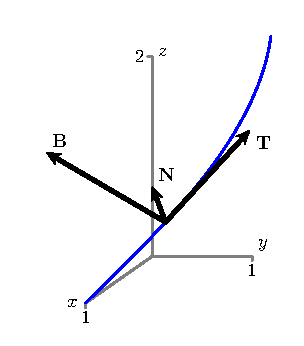
\includegraphics[trim=4.5cm 2.25cm 4.5cm 2.25cm, , clip]{9_8_Ex_4.eps}}
\end{center}
%crop graphics in animate trim=<left> <bottom> <right> <top>,  

	\ea
\end{exerciseSolution}



\item \label{Ez:9.8.5} In this exercise we verify the curvature formula 
\[\kappa = \frac{\lvert \vr'(t) \times \vr''(t) \rvert}{\lvert \vr'(t) \rvert^3}.\]
	\ba
	\item Explain why 
\[\lvert \vr'(t) \rvert = \frac{ds}{dt}.\]

	\item Use the fact that $\vT(t) = \frac{\vr'(t)}{\lvert \vr'(t) \rvert}$ and $\lvert \vr'(t) \rvert = \frac{ds}{dt}$ to explain why 
	\[\vr'(t) = \frac{ds}{dt} \vT(t).\]

	\item The Product Rule shows that 
	\[\vr''(t) = \frac{d^2s}{dt^2} \vT(t) + \frac{ds}{dt} \vT'(t).\]
	Explain why 
	\[\vr'(t) \times \vr''(t) = \left(\frac{ds}{dt}\right)^2 (\vT(t) \times \vT'(t)).\]
	
	\item In Exercise \ref{Ez:9.8.4} we showed that $\lvert \vT(t) \rvert = 1$ implies that $\vT(t)$ is orthogonal to $\vT'(t)$ for every value of $t$. Explain what this tells us about $\lvert \vT(t) \times \vT'(t) \rvert$ and conclude that 
	\[\lvert \vr'(t) \times \vr''(t) \rvert = \left(\frac{ds}{dt}\right)^2 \lvert \vT'(t) \rvert.\]
	
	\item Finally, use the fact that $\kappa = \frac{\lvert \vT'(t) \rvert }{\lvert \vr'(t) \rvert}$ to verify that 
 \[\kappa = \frac{\lvert \vr'(t) \times \vr''(t) \rvert}{\lvert \vr'(t) \rvert^3}.\]
 
	\ea
	
\begin{exerciseSolution}
	\ba
	\item We showed that $\frac{d \vr}{ds} = 1$, so the Chain Rule shows that 
\[\lvert \frac{d \vr}{dt} \rvert = \lvert \frac{d \vr}{ds} \frac{ds}{dt} \rvert = \lvert \frac{d \vr}{ds} \rvert \lvert \frac{ds}{dt} \rvert = \lvert \frac{ds}{dt} \rvert = \frac{ds}{dt},\]
since $s$ is an increasing function. 

	\item Note that 
\[\vr'(t) = \lvert \vr'(t) \rvert \vT(t) = \frac{ds}{dt} \vT(t).\]

	\item Using the previous results we see that 
\begin{align*}
\vr'(t) \times \vr''(t) &= \left( \frac{ds}{dt} \vT(t) \right) \times \left( \frac{d^2s}{dt^2} \vT(t) + \frac{ds}{dt} \vT'(t) \right) \\
	&= \left( \frac{ds}{dt} \vT(t) \times \frac{d^2s}{dt^2} \vT(t) \right) + \left( \frac{ds}{dt} \vT(t) \times \frac{ds}{dt} \vT'(t) \right) \\
	&= \left( \frac{ds}{dt} \right) \left( \frac{d^2s}{dt^2} \right) \left( \vT(t) \times \vT(t) \right) + \left( \frac{ds}{dt} \right) \left( \frac{ds}{dt} \right) \left( \vT(t) \times \vT'(t) \right) \\
	&= \left(\frac{ds}{dt}\right)^2 (\vT(t) \times \vT'(t)).
\end{align*}

	\item We know that 
\[\vT(t) \times \vT'(t) = \lvert \vT(t) \rvert \lvert \vT'(t) \rvert \sin\left(\frac{\pi}{2}\right) \vn\]
for some unit vector $\vn$ orthogonal to both $\vT(t)$ and $\vT'(t)$. So 
\[\lvert \vT(t) \times \vT'(t) \rvert = \lvert \vT(t) \rvert \lvert \vT'(t) \rvert \sin\left(\frac{\pi}{2}\right) \lvert \vn \rvert = \lvert \vT'(t) \rvert.\]
It follows that 
\[\lvert \vr'(t) \times \vr''(t) \rvert = \left(\frac{ds}{dt}\right)^2 \lvert \vT(t) \times \vT'(t) \rvert = \left(\frac{ds}{dt}\right)^2 \lvert \vT'(t) \rvert.\]

	\item We have 
 \[\lvert \vT'(t) \rvert = \frac{\lvert \vr'(t) \times \vr''(t) \rvert}{\left(\frac{ds}{dt}\right)^2}\]
 and so
 \begin{align*}
\kappa &= \frac{\lvert \vT'(t) \rvert }{\lvert \vr'(t) \rvert} \\
	&= \frac{\lvert \vr'(t) \times \vr''(t) \rvert }{\left(\frac{ds}{dt}\right)^2 \lvert \vr'(t) \rvert} \\
	&= \frac{\lvert \vr'(t) \times \vr''(t) \rvert }{\left( \lvert \vr'(t) \rvert \right)^2 \lvert \vr'(t) \rvert} \\
	&= \frac{\lvert \vr'(t) \times \vr''(t) \rvert}{\lvert \vr'(t) \rvert^3}.
\end{align*}

	\ea
\end{exerciseSolution}


\end{exercises}

\afterexercises
